% !TeX encoding = UTF-8 
% !TeX spellcheck = de_DE 
% !TeX program = pdflatex
% !BIB program = biber
\documentclass{wab}

%TODO bitte hier die Matrikelnummer und Gruppe angeben
\institute{Matrikel: DKMI17}

\authors{Marvin Laubenstein}{Marc Hey}{}{}
\contactperson{s176137@hft-leipzig.de}
\title{MF02 S-Parameter VNA}



\handindate{\today}


\bibliography{References/rfc,References/ieee,References/itut,References/3gpp,References/etsi,References/w3c,References/online, References/quellen}

\begin{document}


\maketitle

\pagenumbering{Roman}
\newpage

\cleardoublepage

\tableofcontents
\cleardoublepage
\phantomsection
\listoffigures


% Bei Bedarf auskommentieren
%\lstlistoflistings
%\addcontentsline{toc}{chapter}{Quellcodeverzeichnis}

\clearpage
\newpage
\section*{Abkürzungsverzeichnis}

\markboth{\footnotesize{Abkürzungsverzeichnis}}{\footnotesize{Abkürzungsverzeichnis}}
\addcontentsline{toc}{section}{Abkürzungsverzeichnis}
	
\begin{acronym}[ABCDEF]
\acro{SWR}{Standing Wave Ratio (Stehwellenverhältnis)}
\acro{VNA}{Vektorieller Netzwerkanalysator}
\acro{S Parameter}{Streuparameter}
\acro{DUT}{Device Under Test}

\end{acronym}

\clearpage
\section*{Versuchsanleitung}
\markboth{\footnotesize{Versuchsanleitung}}{\footnotesize{Versuchsanleitung}}
\addcontentsline{toc}{section}{Versuchsanleitung}

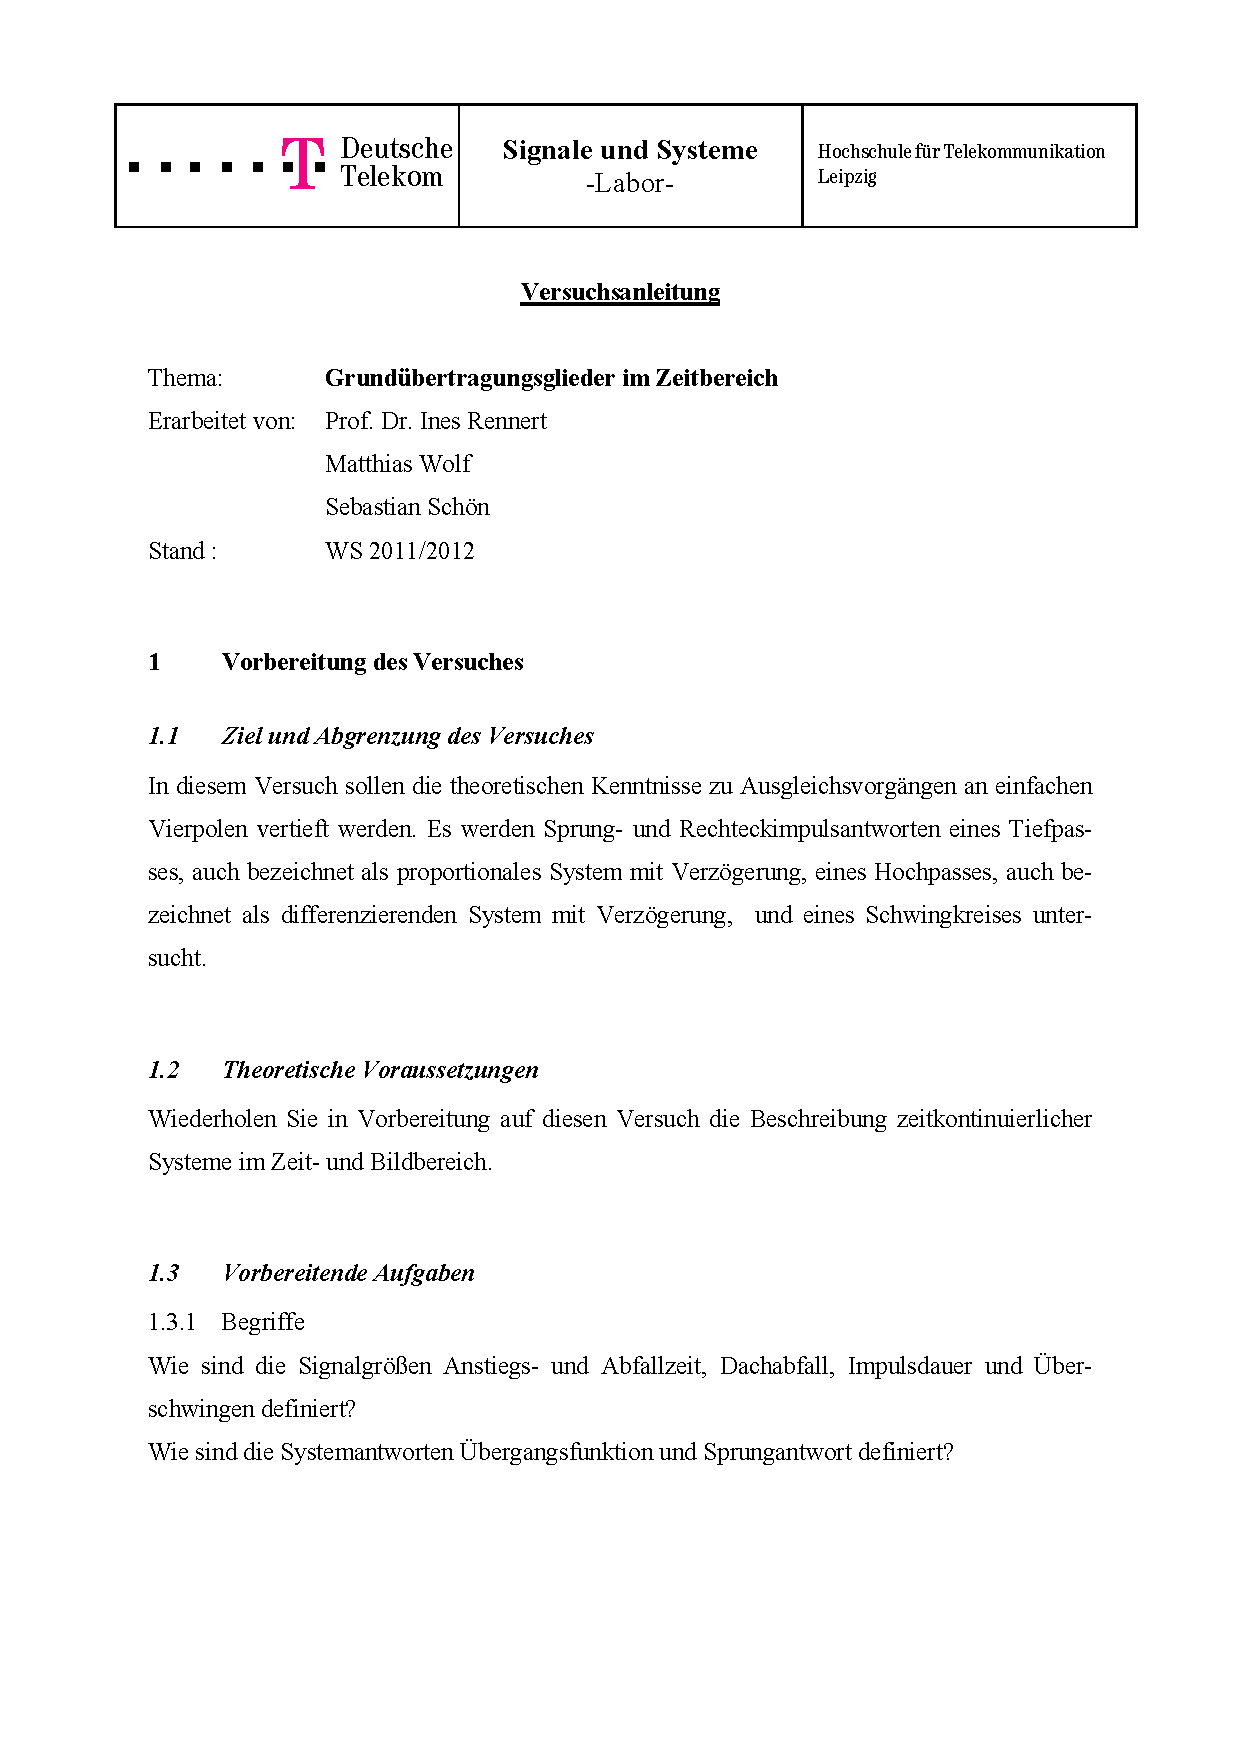
\includegraphics[width=1.0\textwidth]{Bilder/Grundubertragungsglieder im Zeitbereich (verschoben)}\newpage
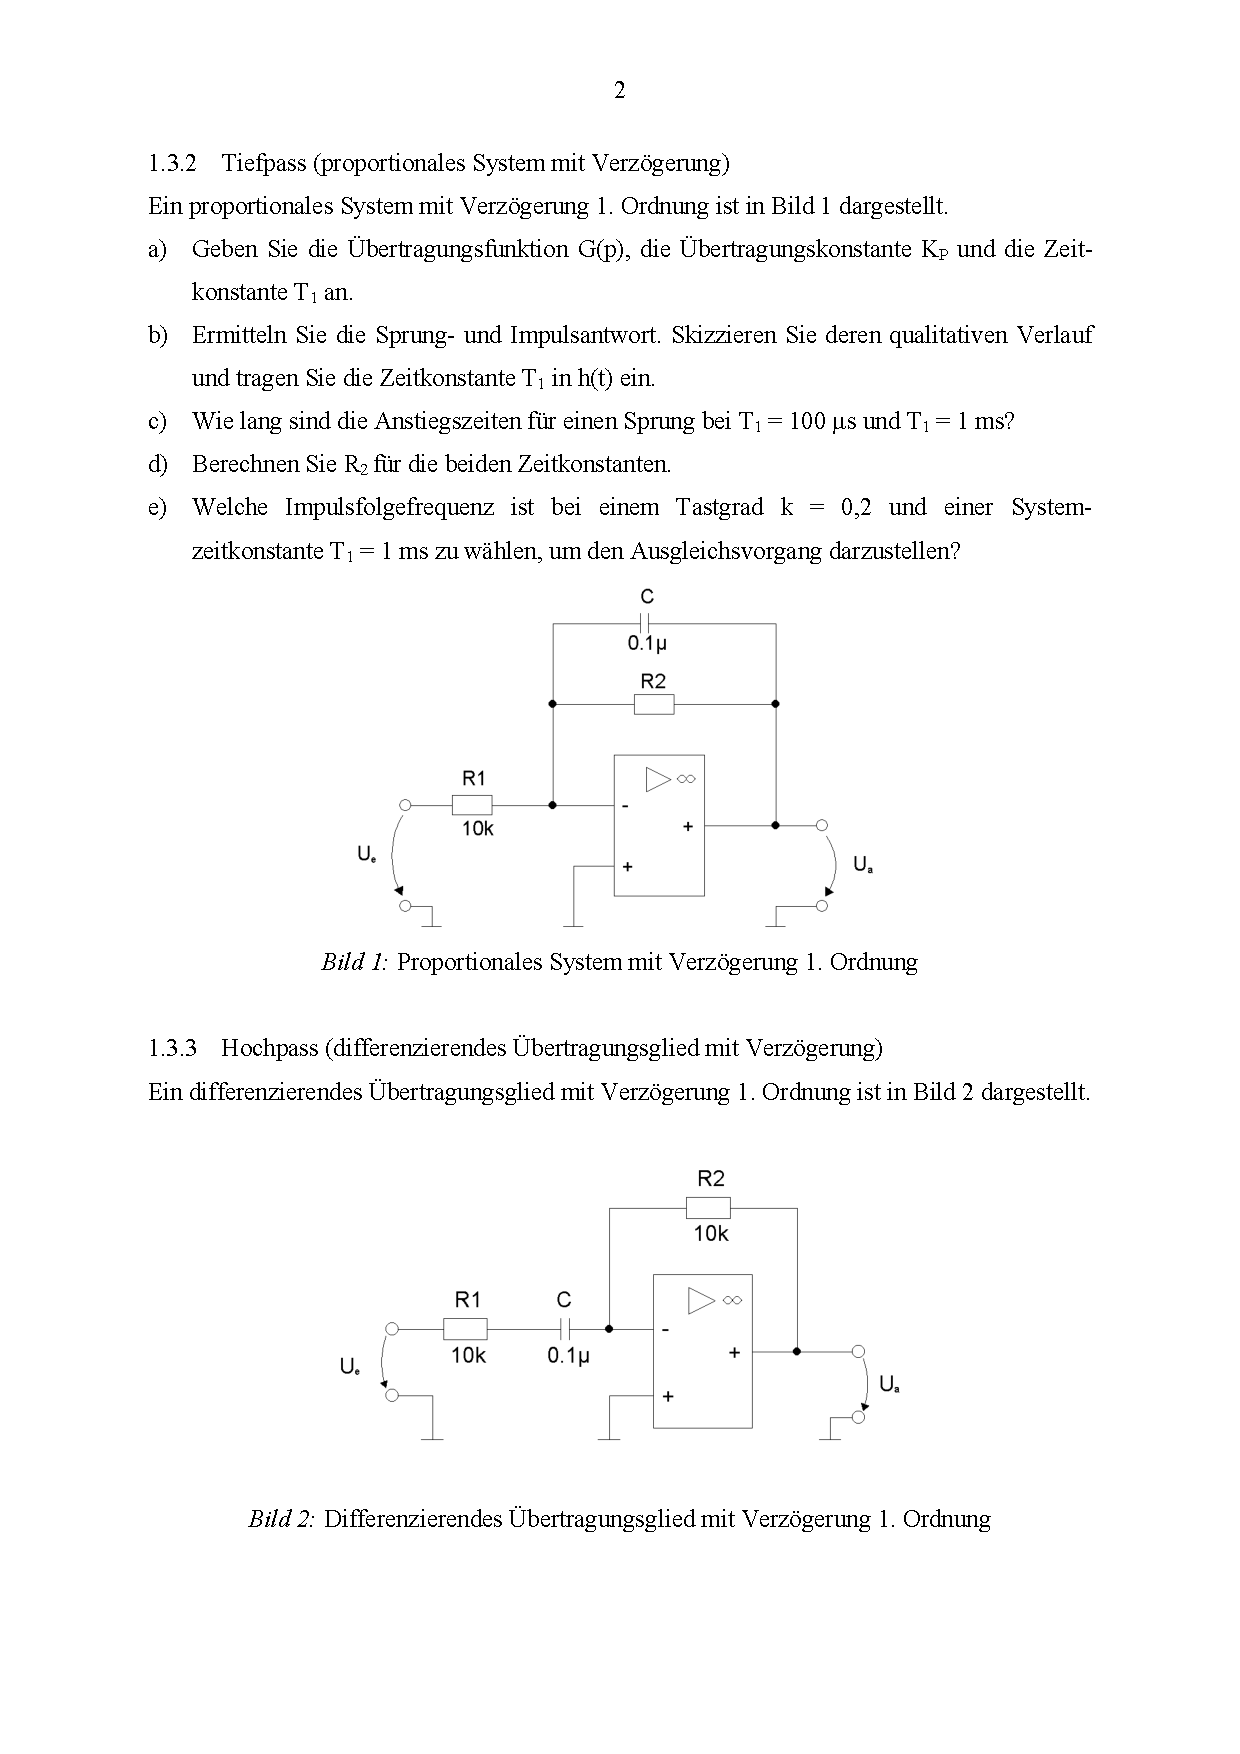
\includegraphics[width=1.0\textwidth]{Bilder/Grundubertragungsglieder im Zeitbereich (verschoben) 2}\newpage
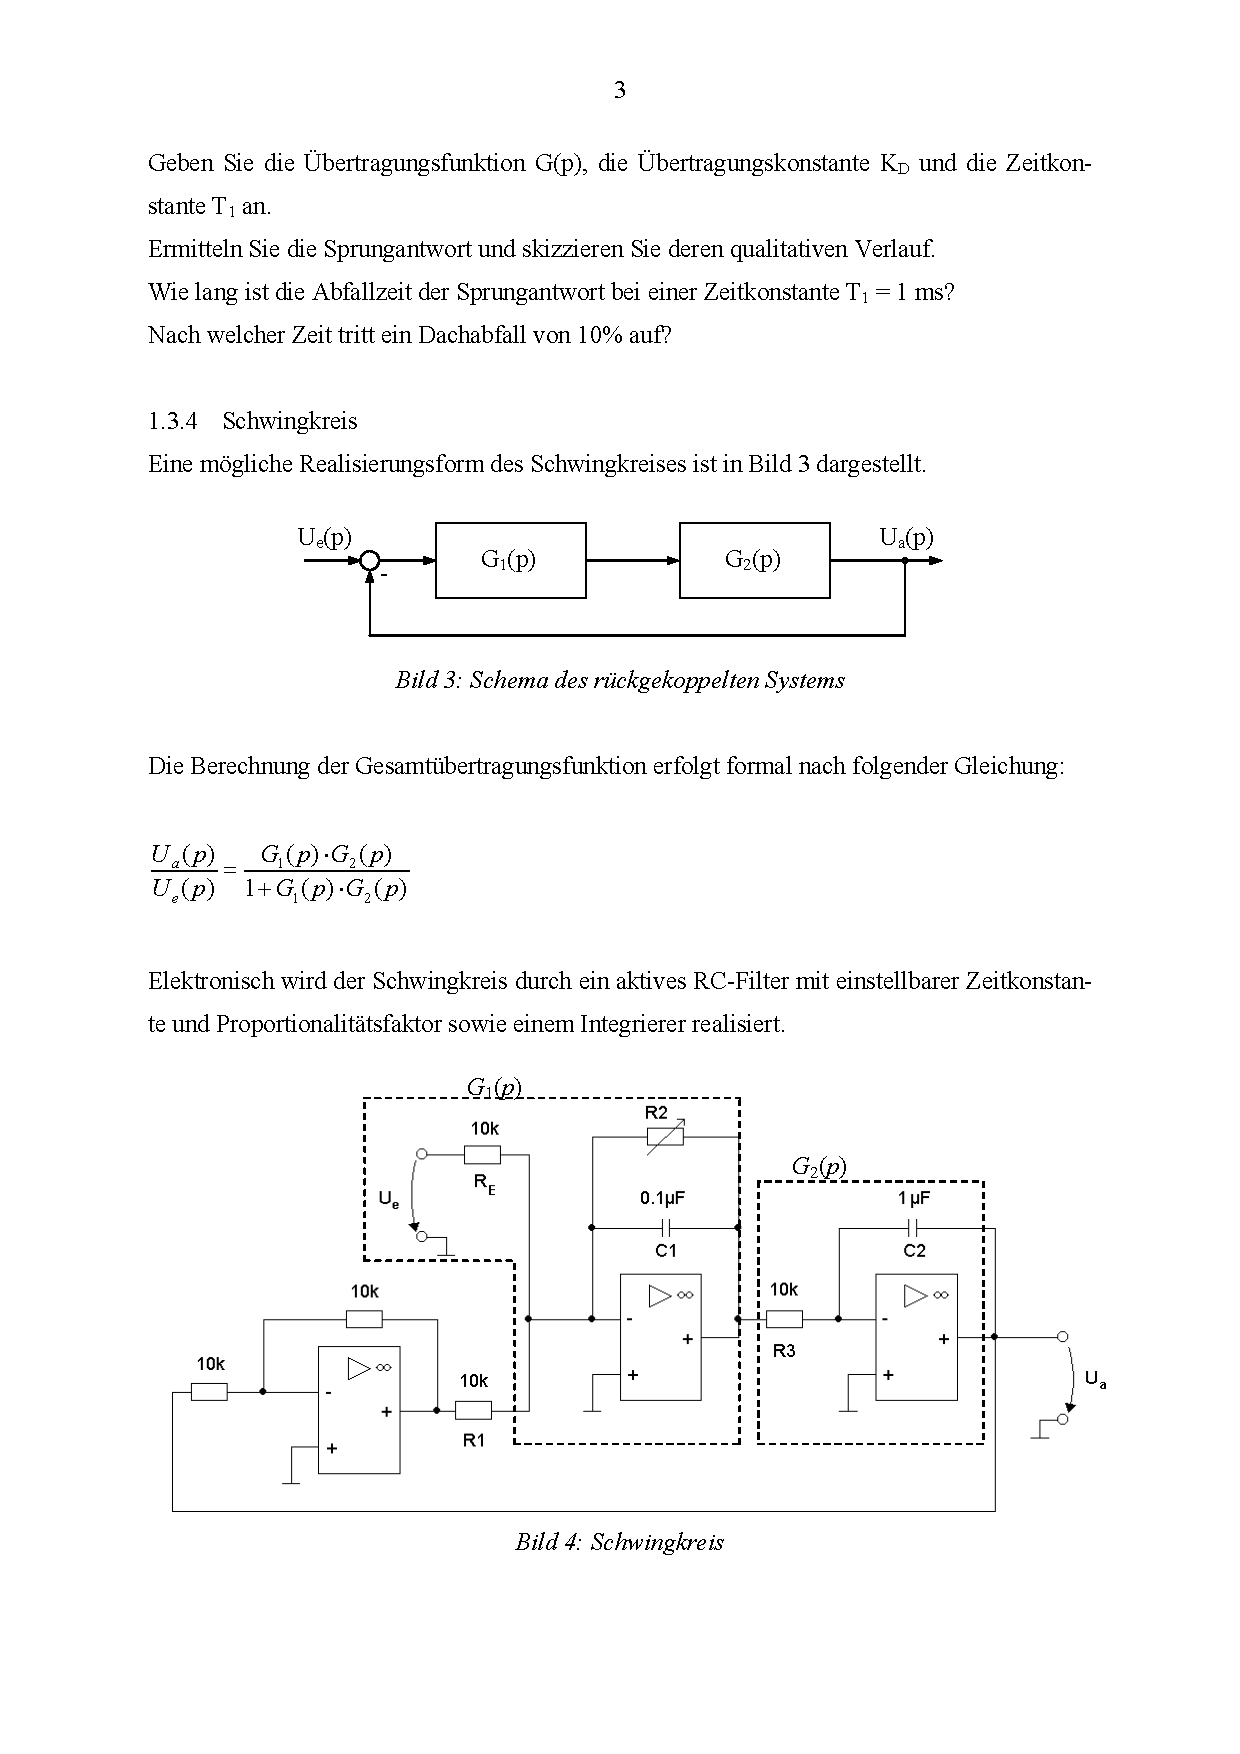
\includegraphics[width=1.0\textwidth]{Bilder/Grundubertragungsglieder im Zeitbereich (verschoben) 3}\newpage
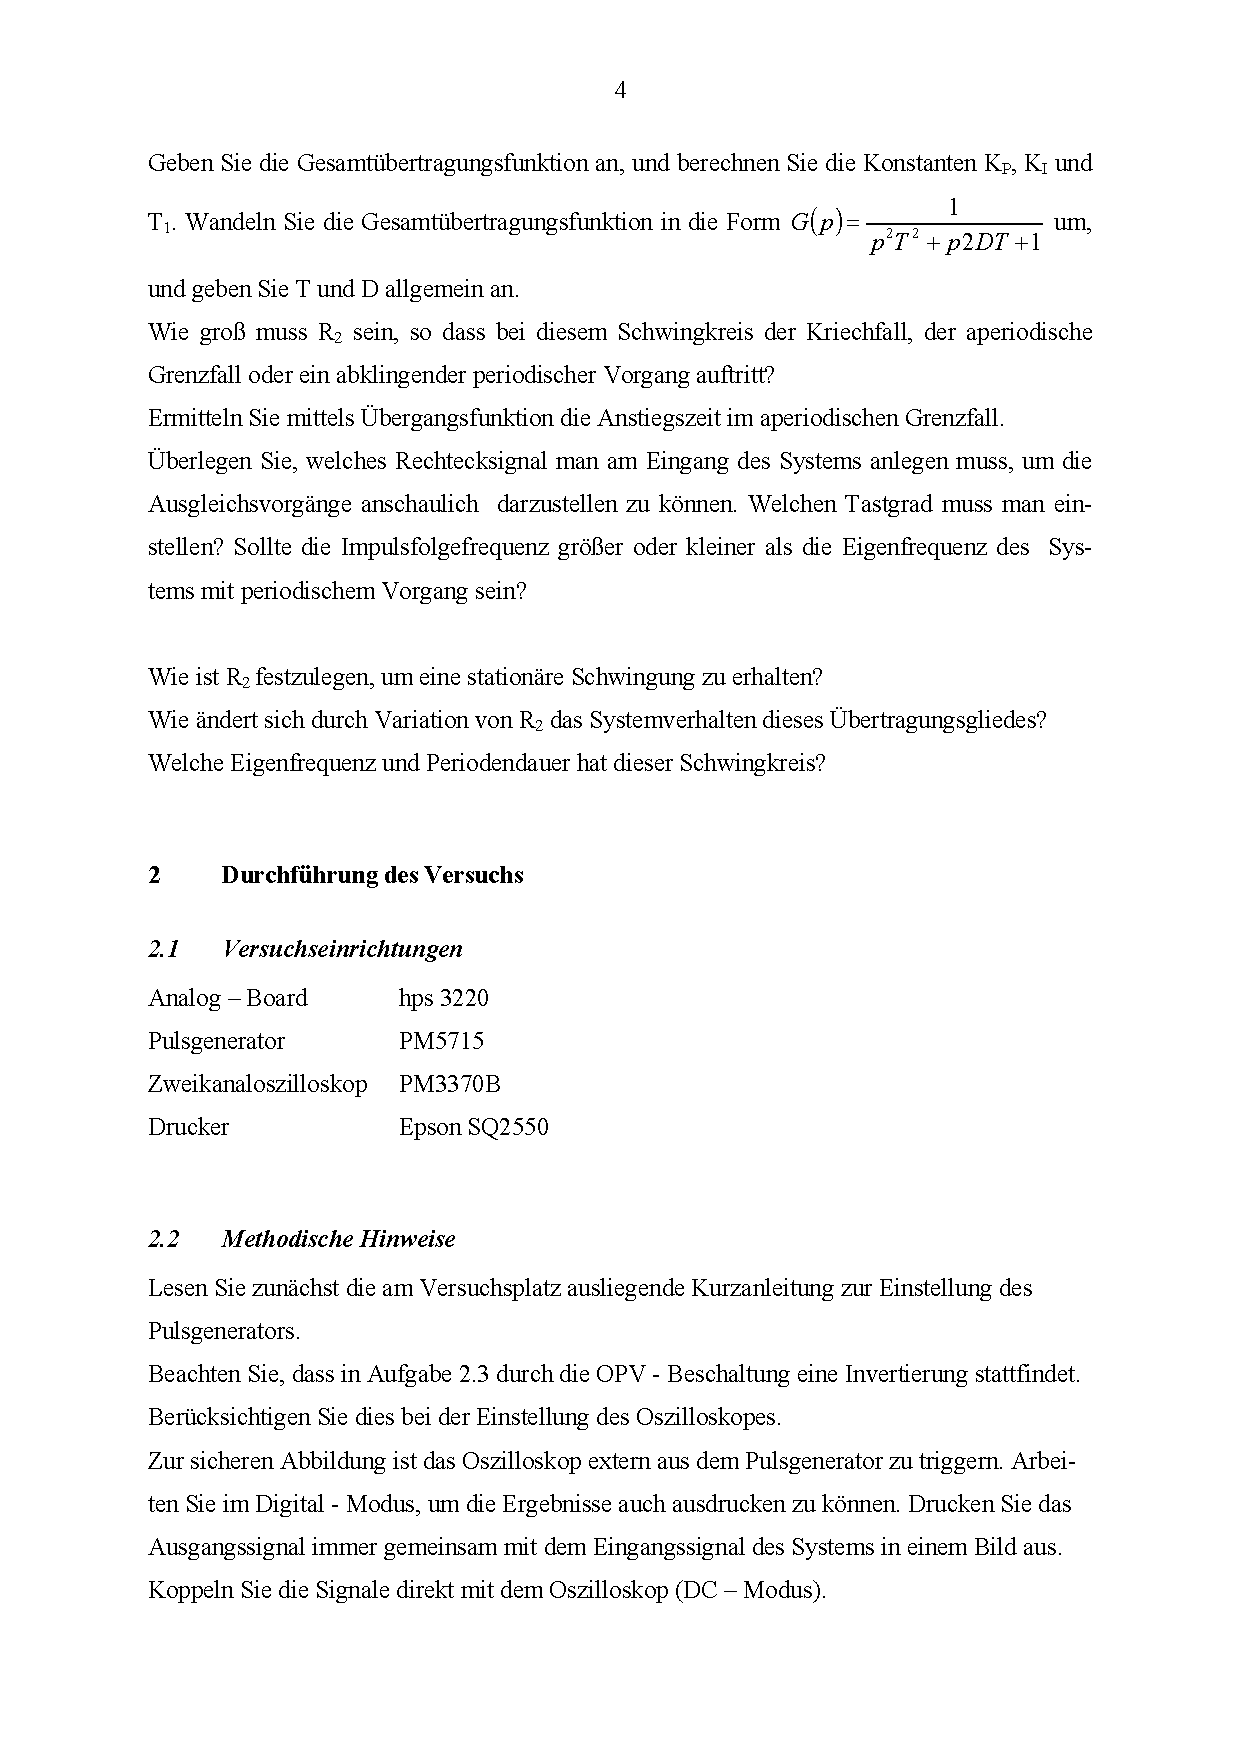
\includegraphics[width=1.0\textwidth]{Bilder/Grundubertragungsglieder im Zeitbereich (verschoben) 4}\newpage
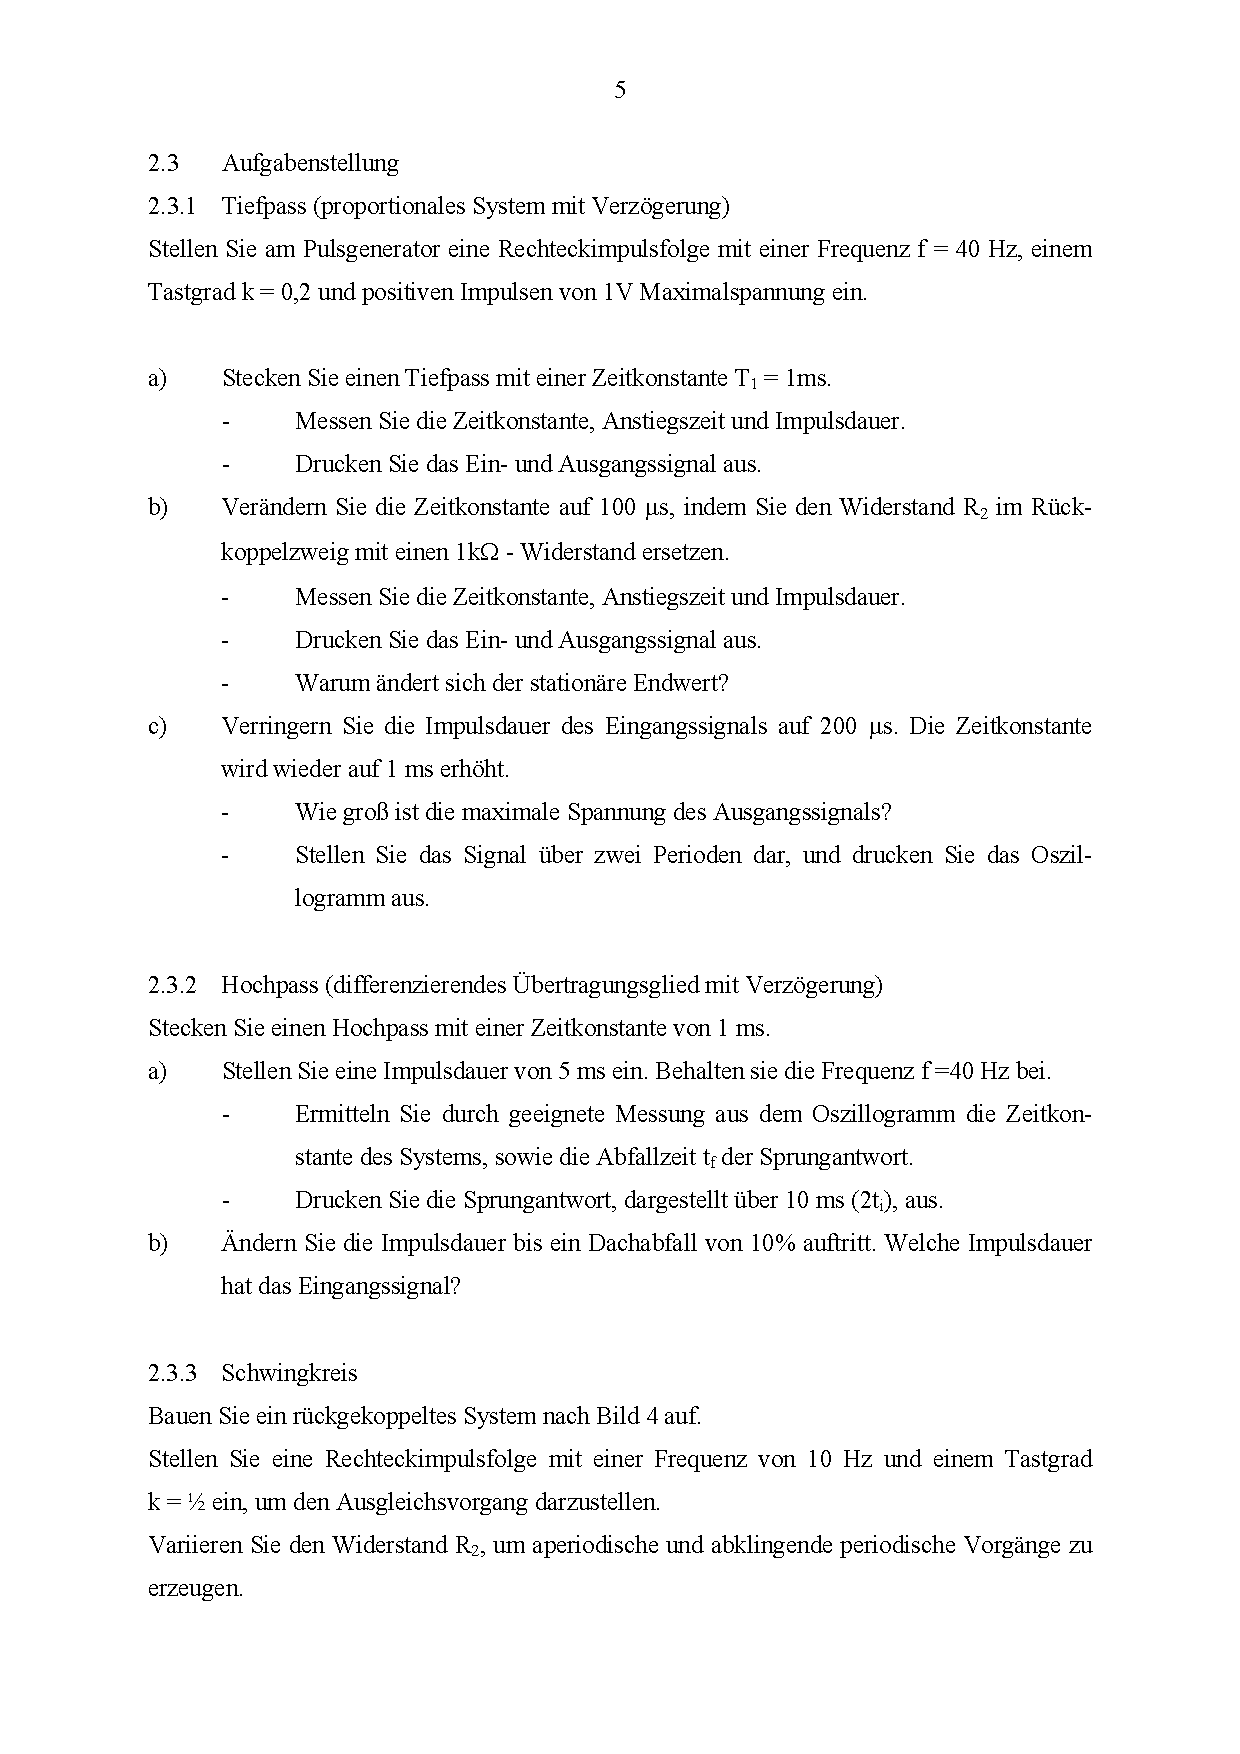
\includegraphics[width=1.0\textwidth]{Bilder/Grundubertragungsglieder im Zeitbereich (verschoben) 5}\newpage
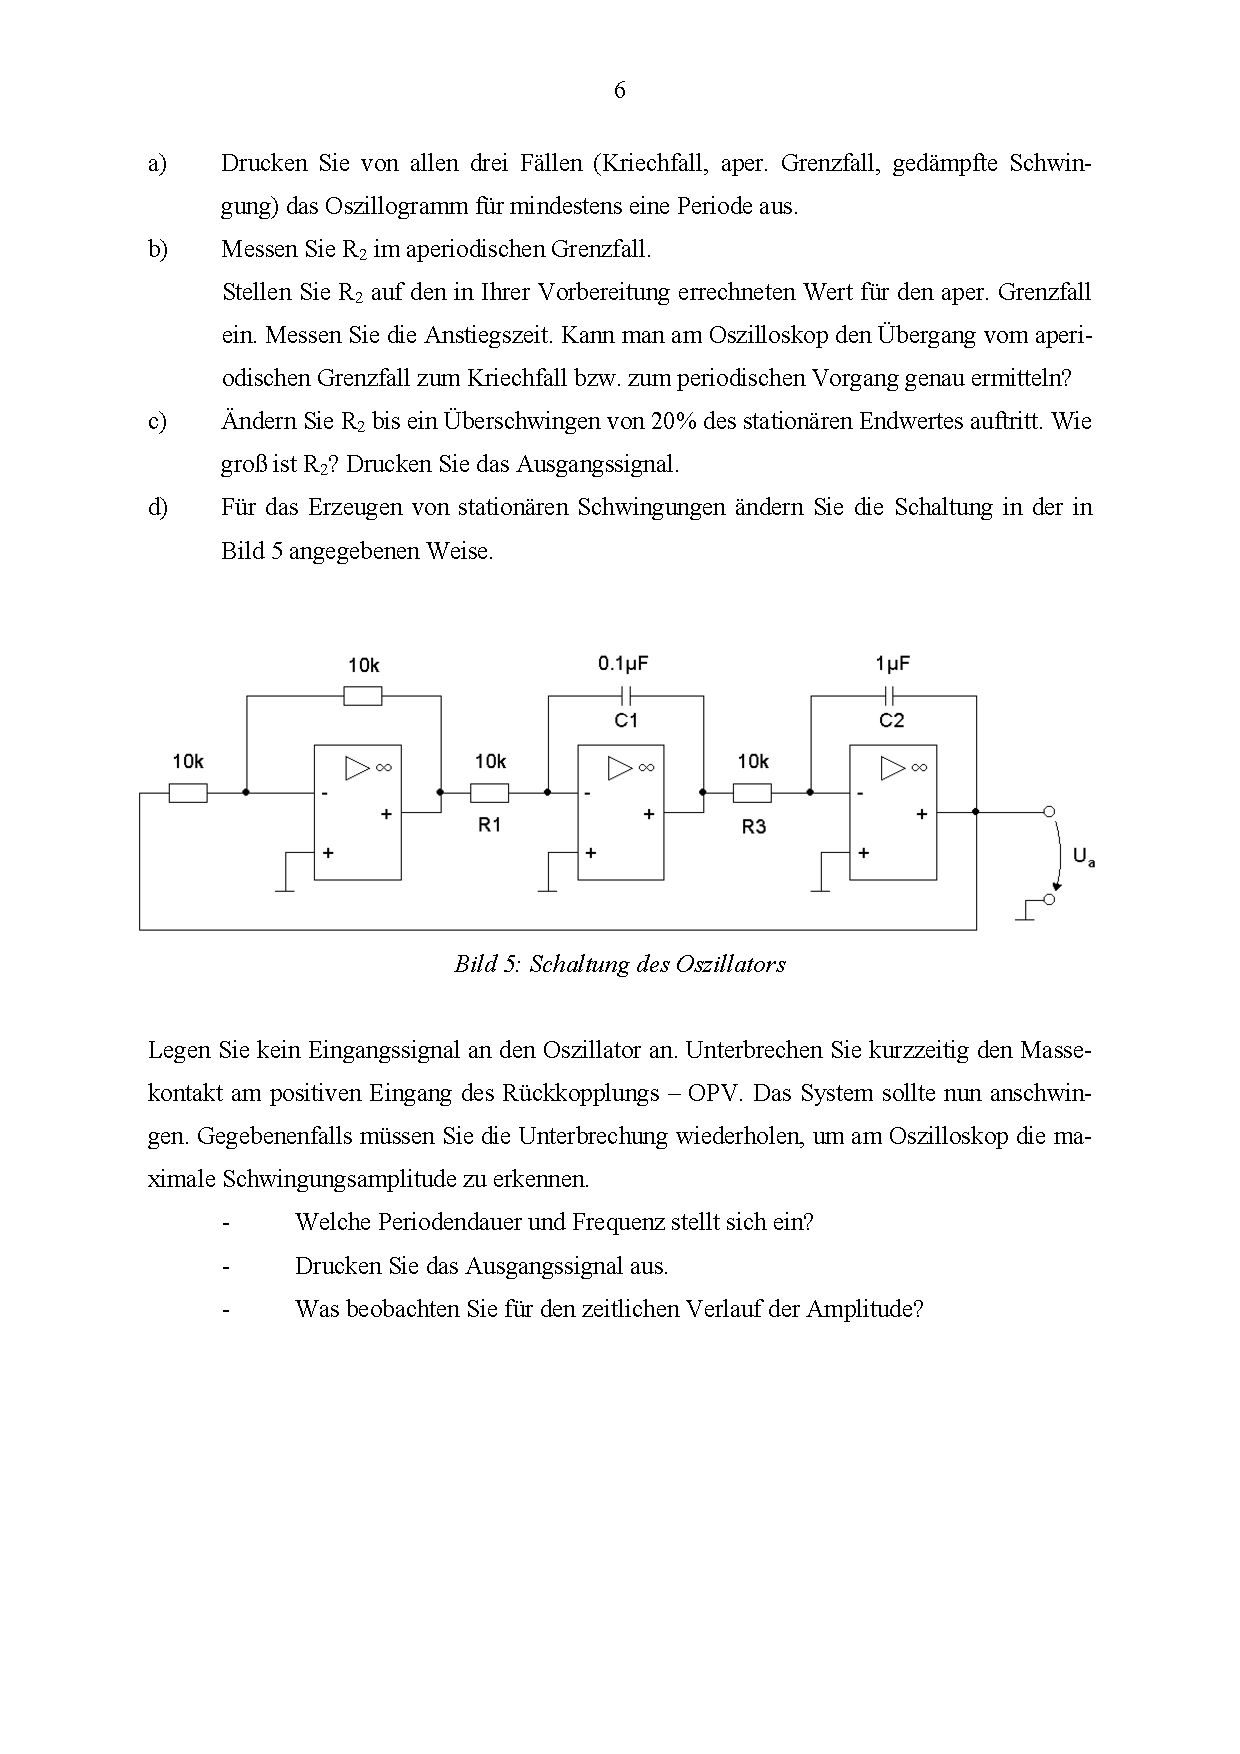
\includegraphics[width=1.0\textwidth]{Bilder/Grundubertragungsglieder im Zeitbereich (verschoben) 6}\newpage
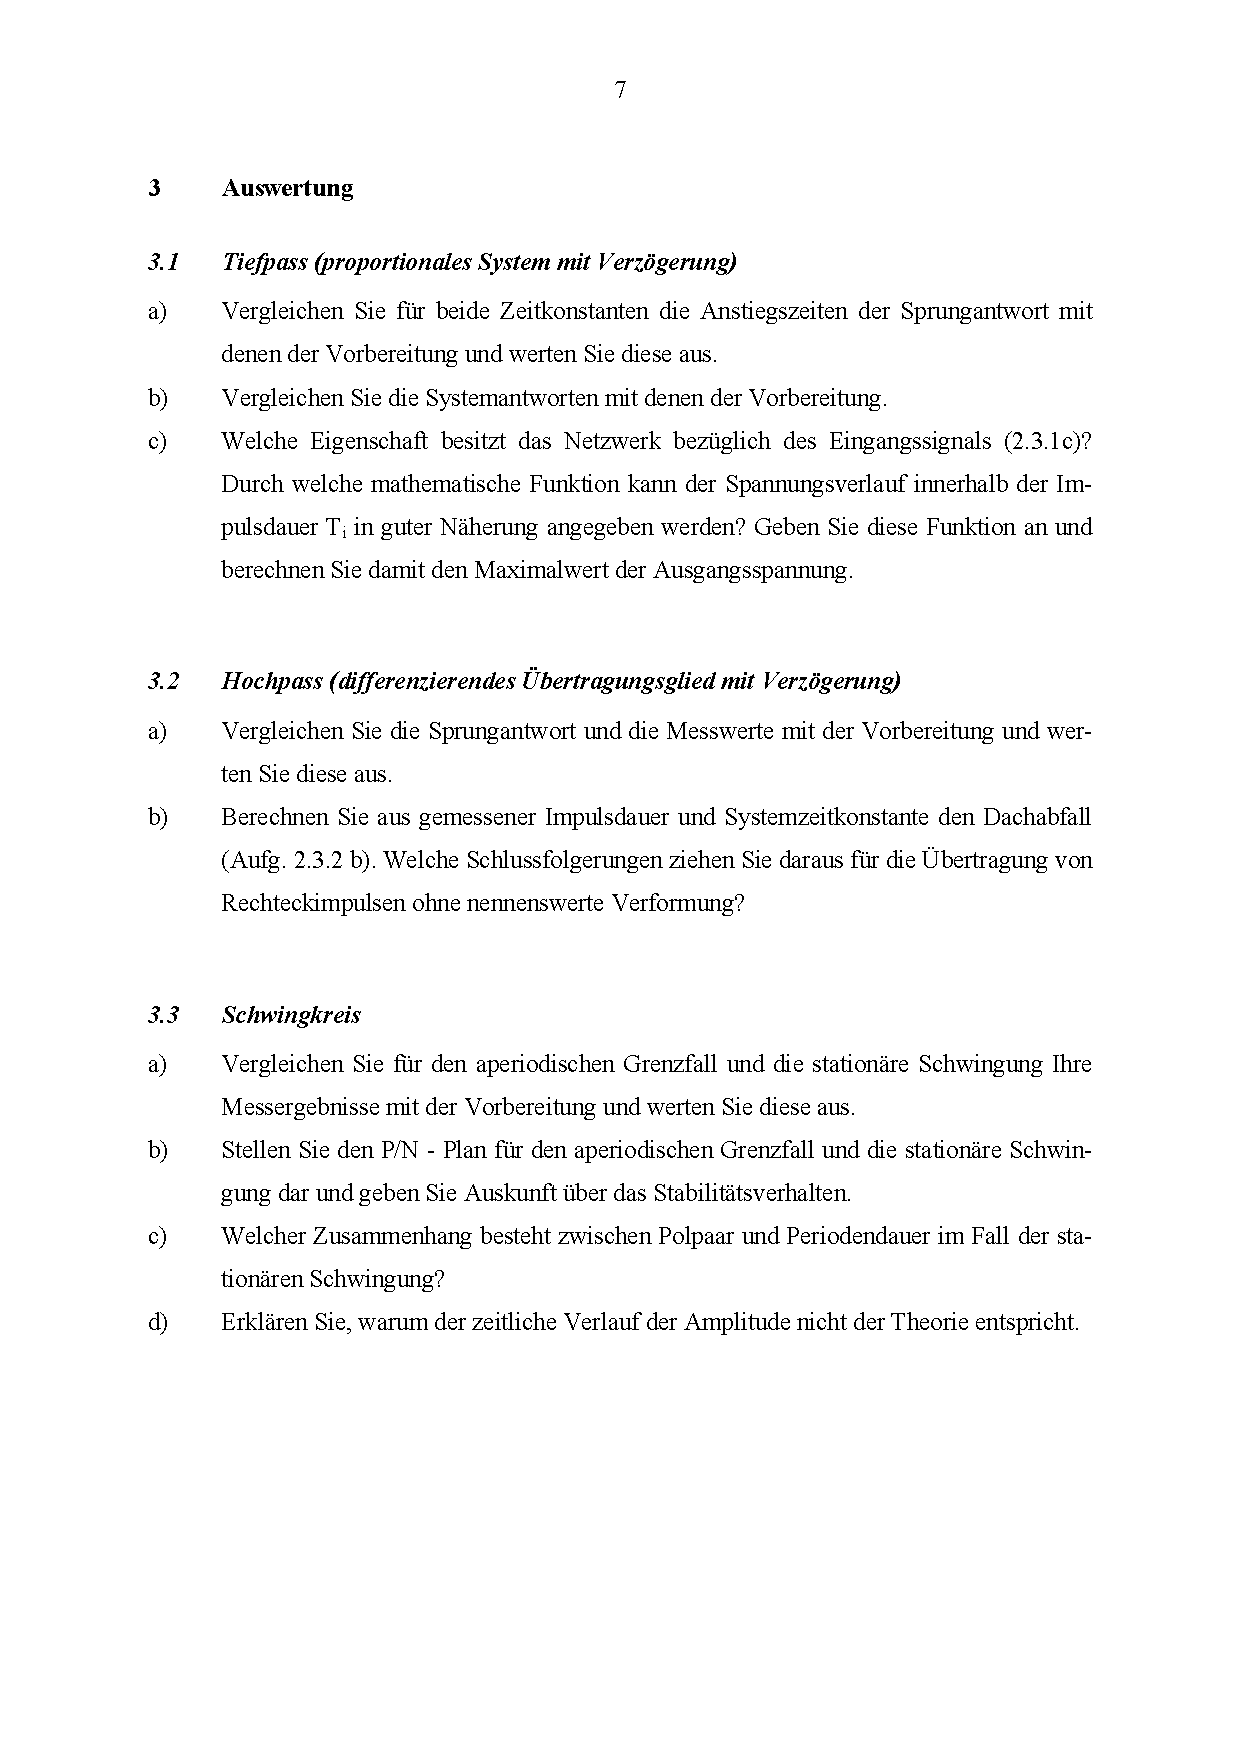
\includegraphics[width=1.0\textwidth]{Bilder/Grundubertragungsglieder im Zeitbereich (verschoben) 7}\newpage




\pagenumbering{arabic}
\setcounter{page}{1}

%Einbinden des ersten Kapitels
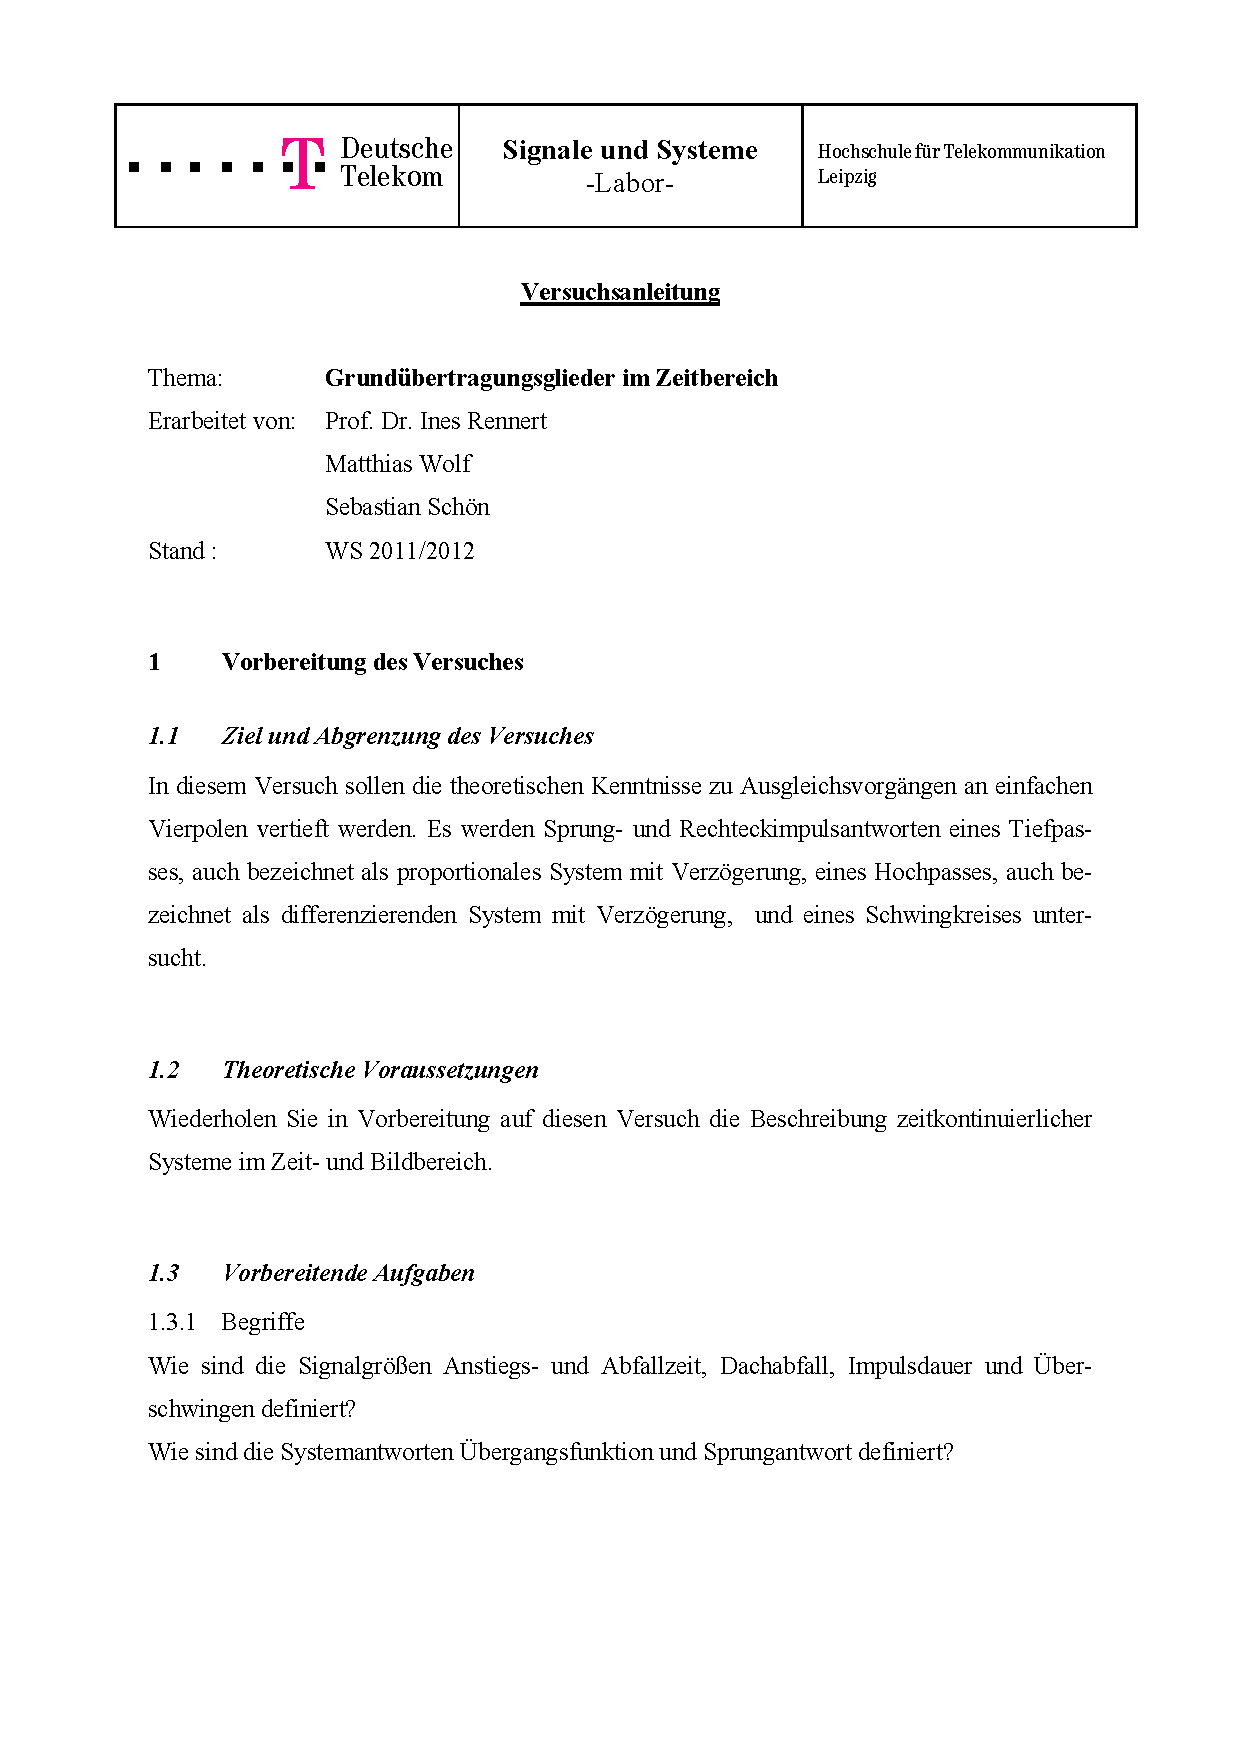
\includegraphics[width=1.0\textwidth]{Bilder/Grundubertragungsglieder im Zeitbereich (verschoben)}\newpage
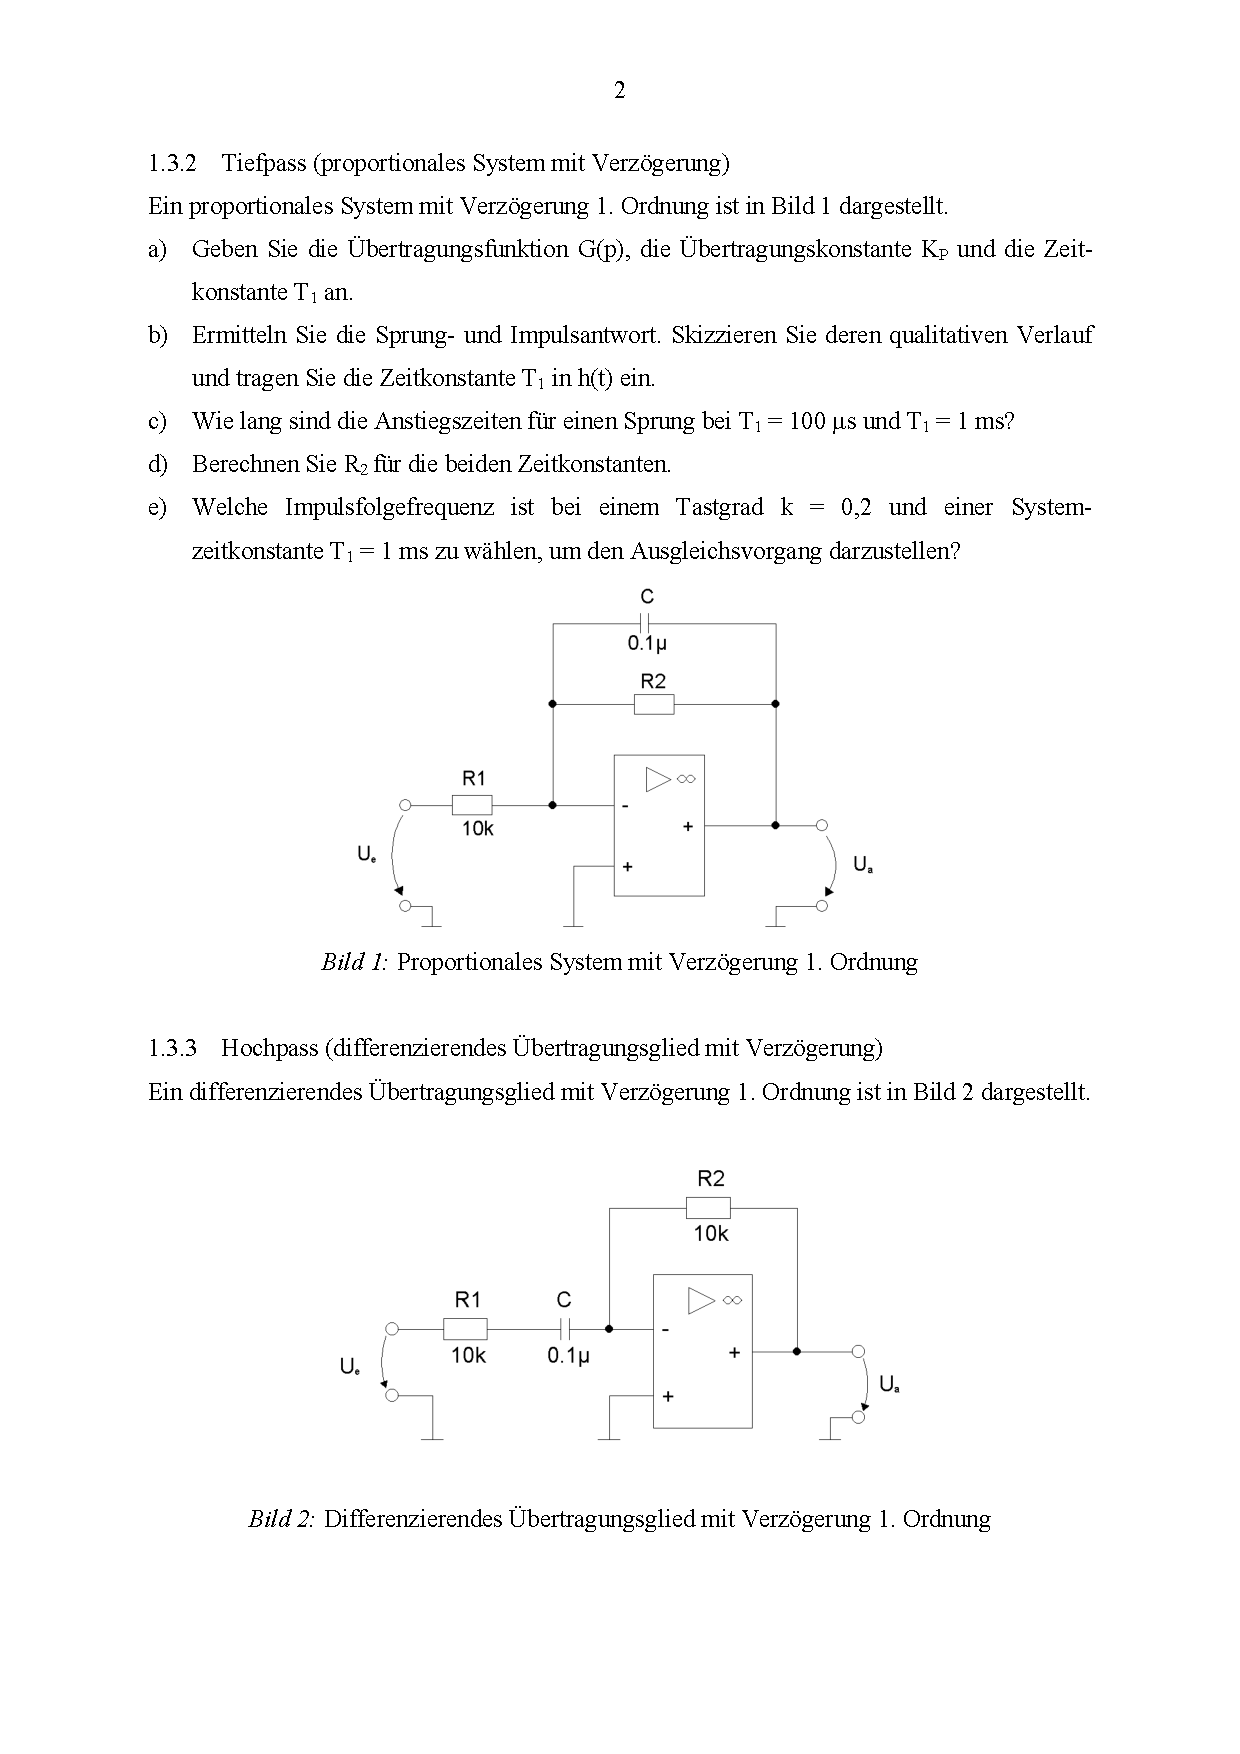
\includegraphics[width=1.0\textwidth]{Bilder/Grundubertragungsglieder im Zeitbereich (verschoben) 2}\newpage
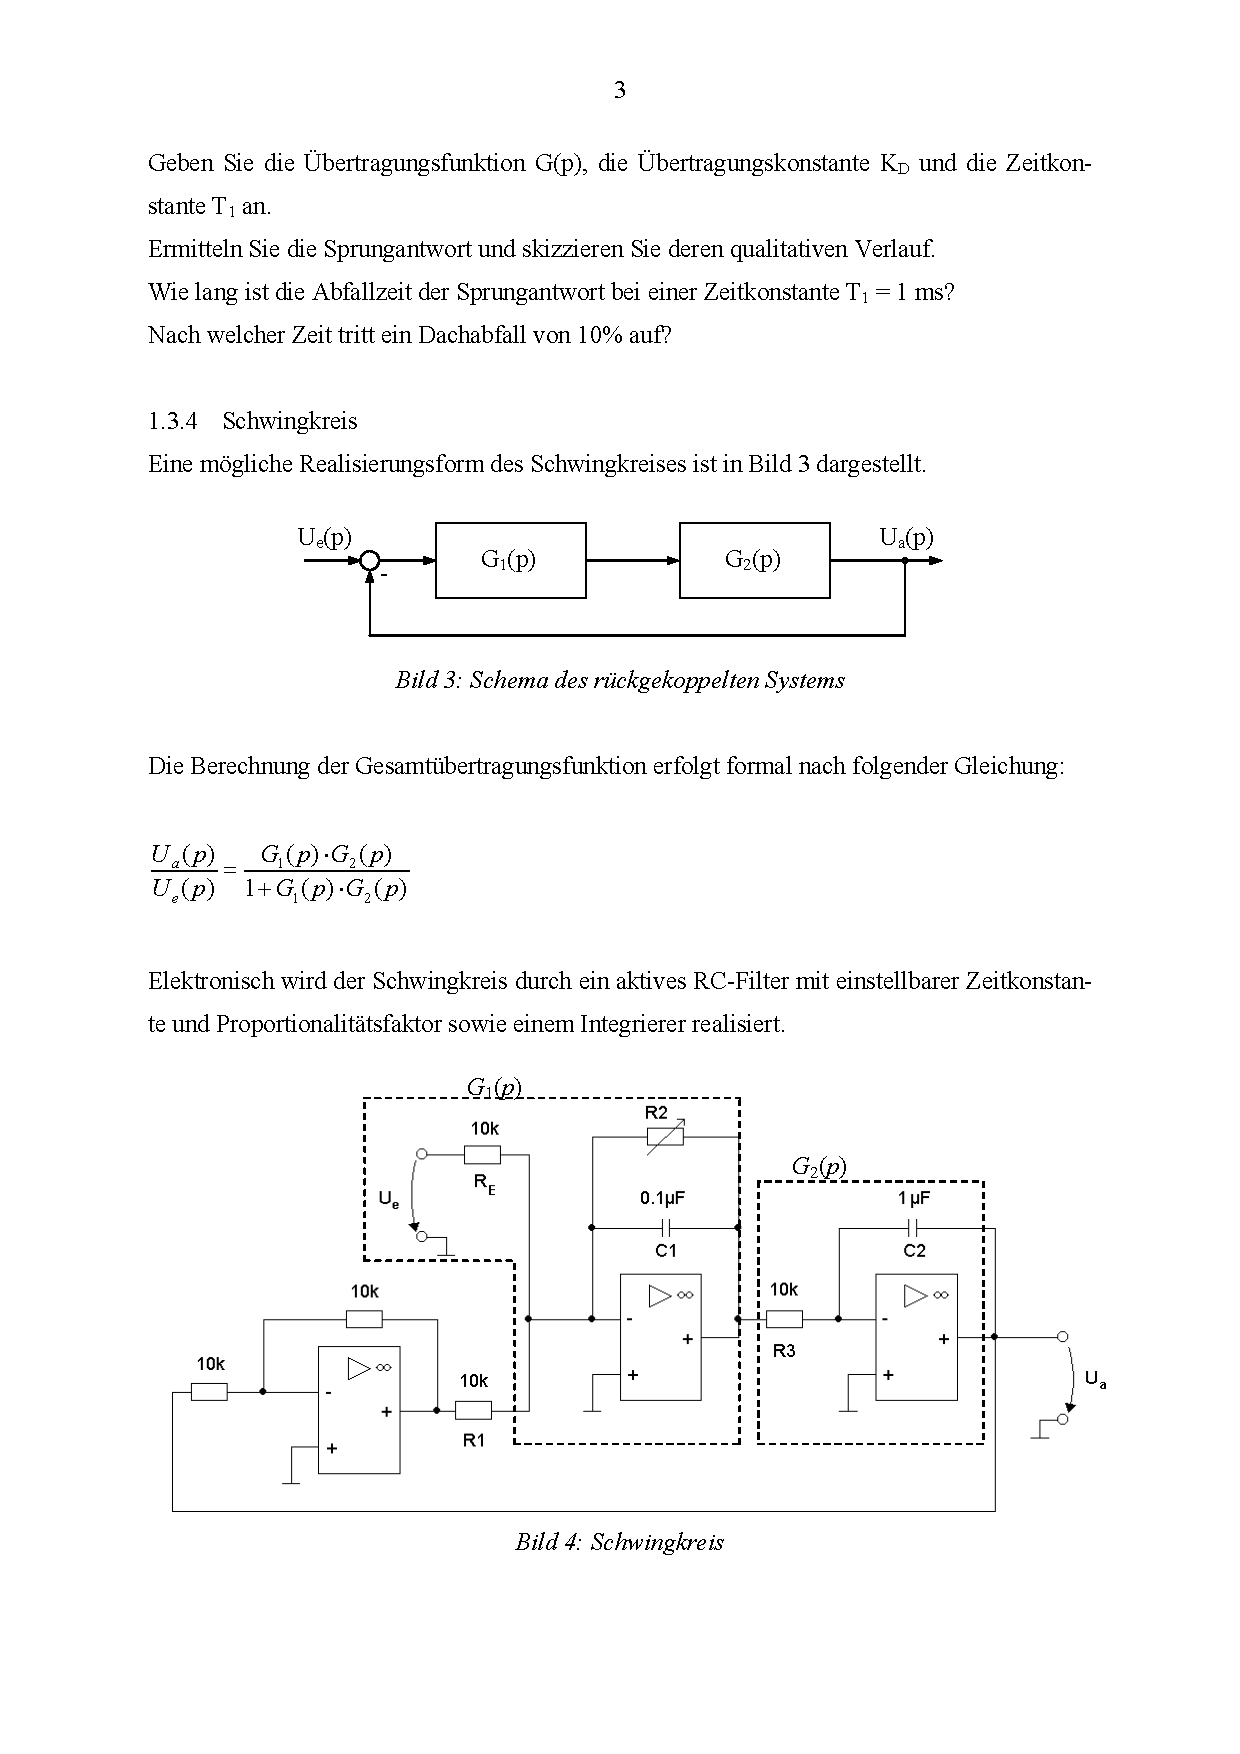
\includegraphics[width=1.0\textwidth]{Bilder/Grundubertragungsglieder im Zeitbereich (verschoben) 3}\newpage
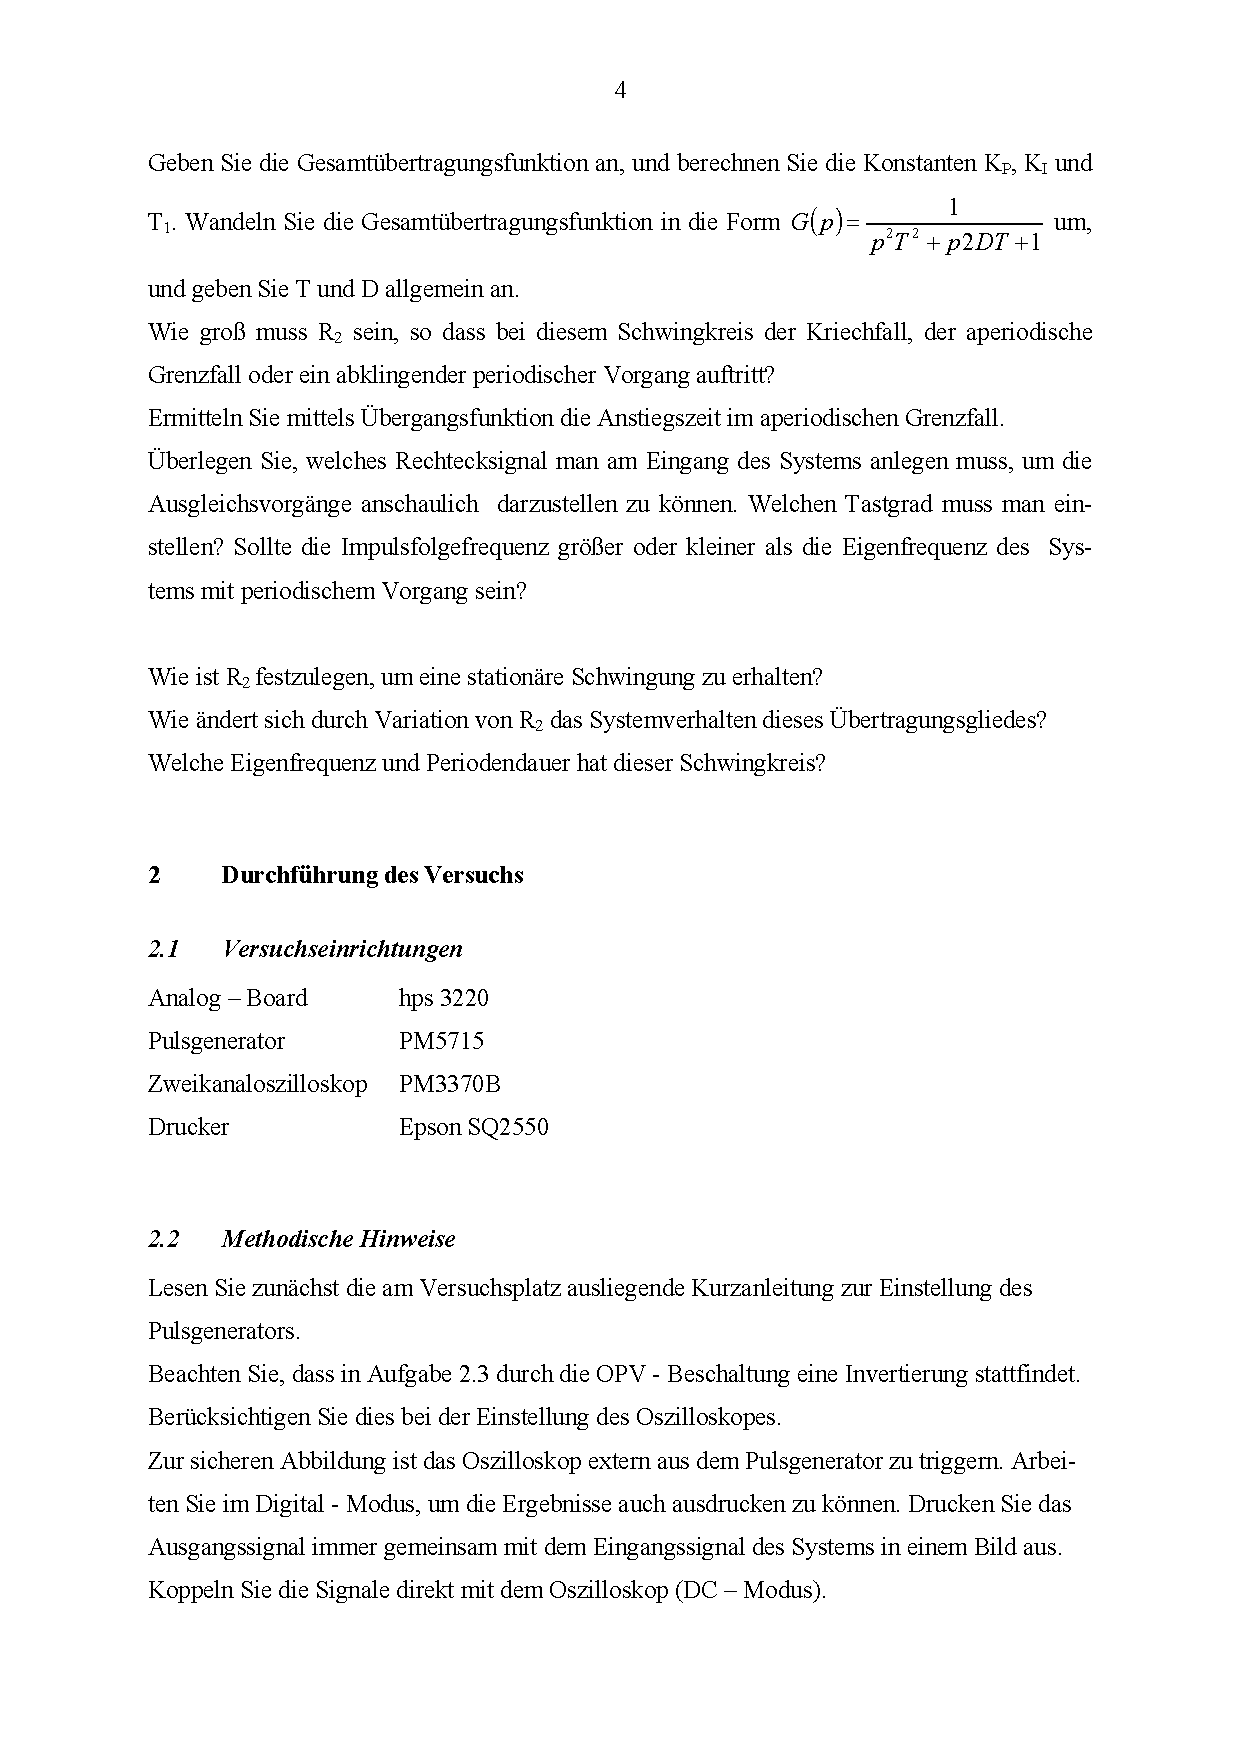
\includegraphics[width=1.0\textwidth]{Bilder/Grundubertragungsglieder im Zeitbereich (verschoben) 4}\newpage
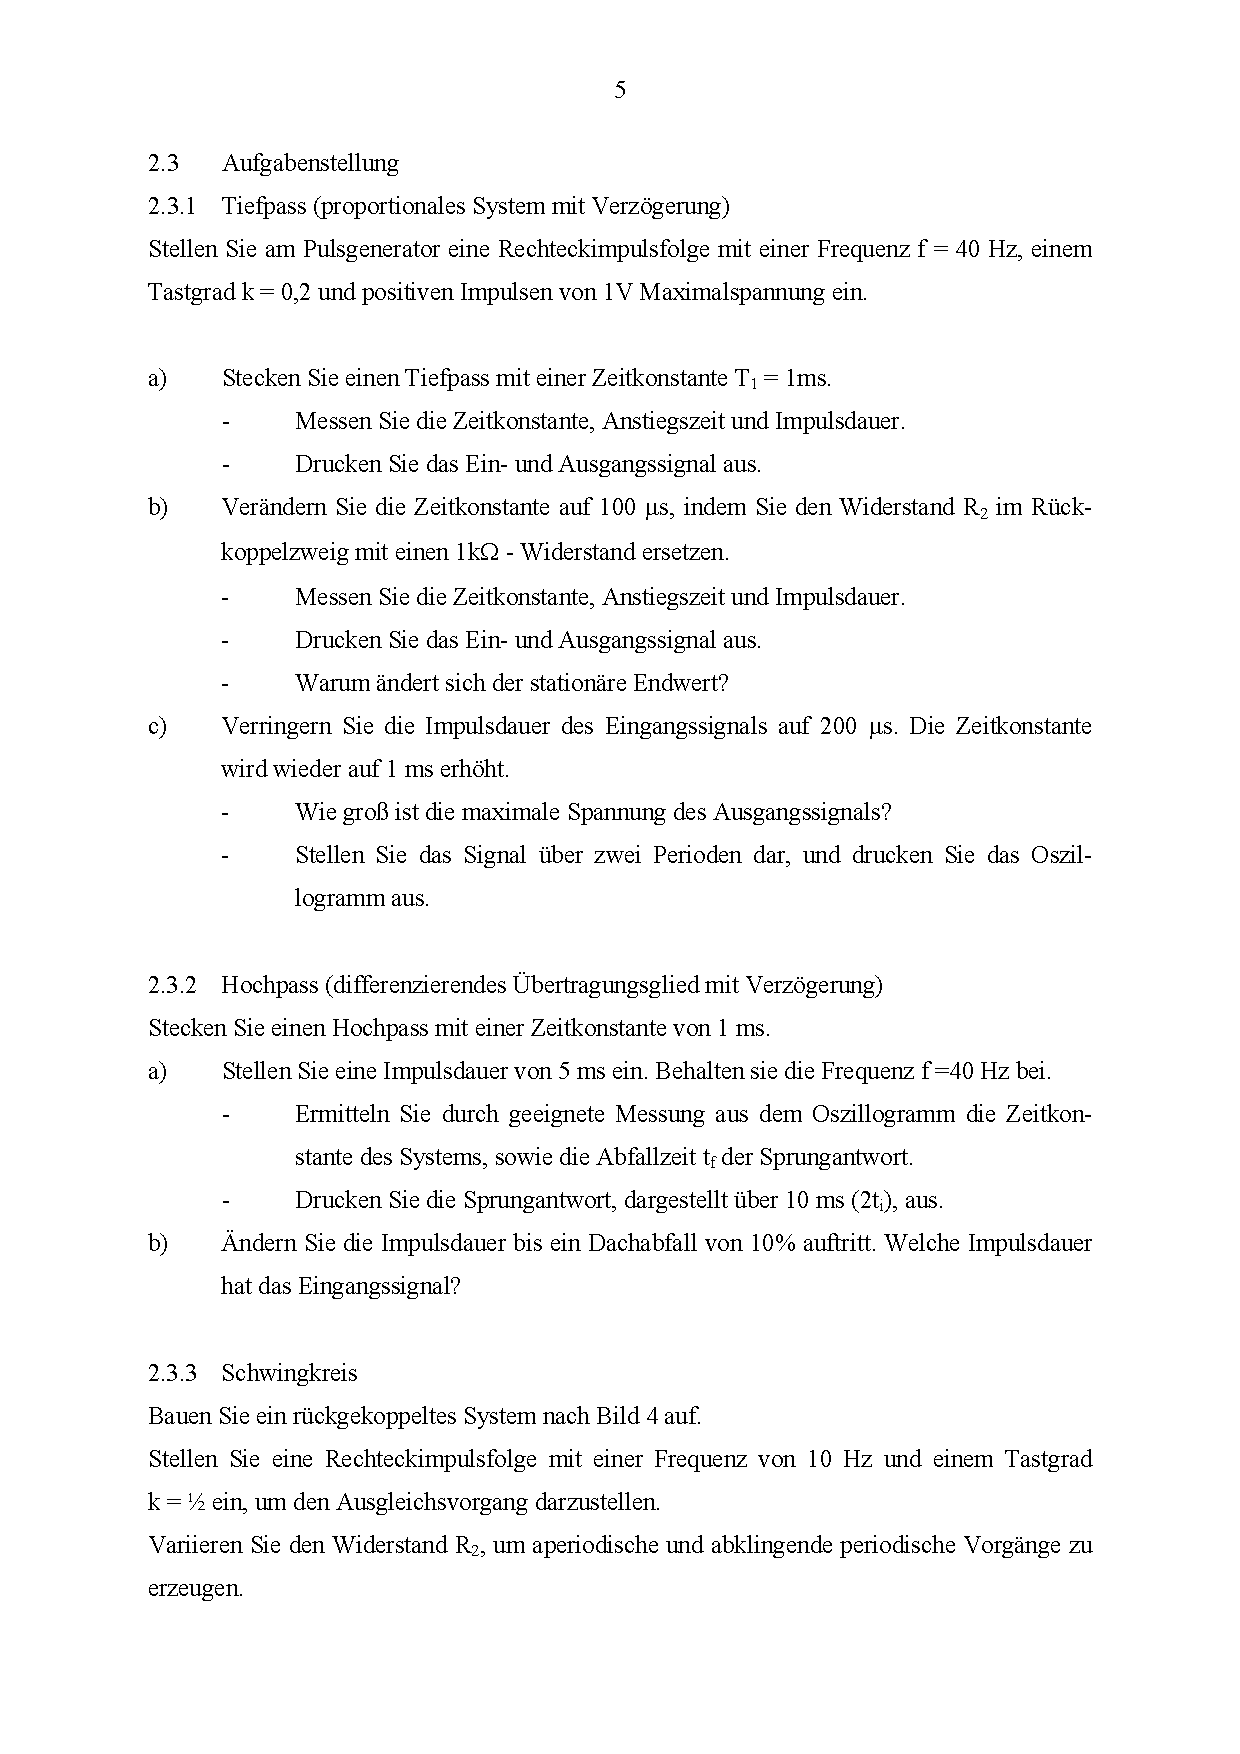
\includegraphics[width=1.0\textwidth]{Bilder/Grundubertragungsglieder im Zeitbereich (verschoben) 5}\newpage
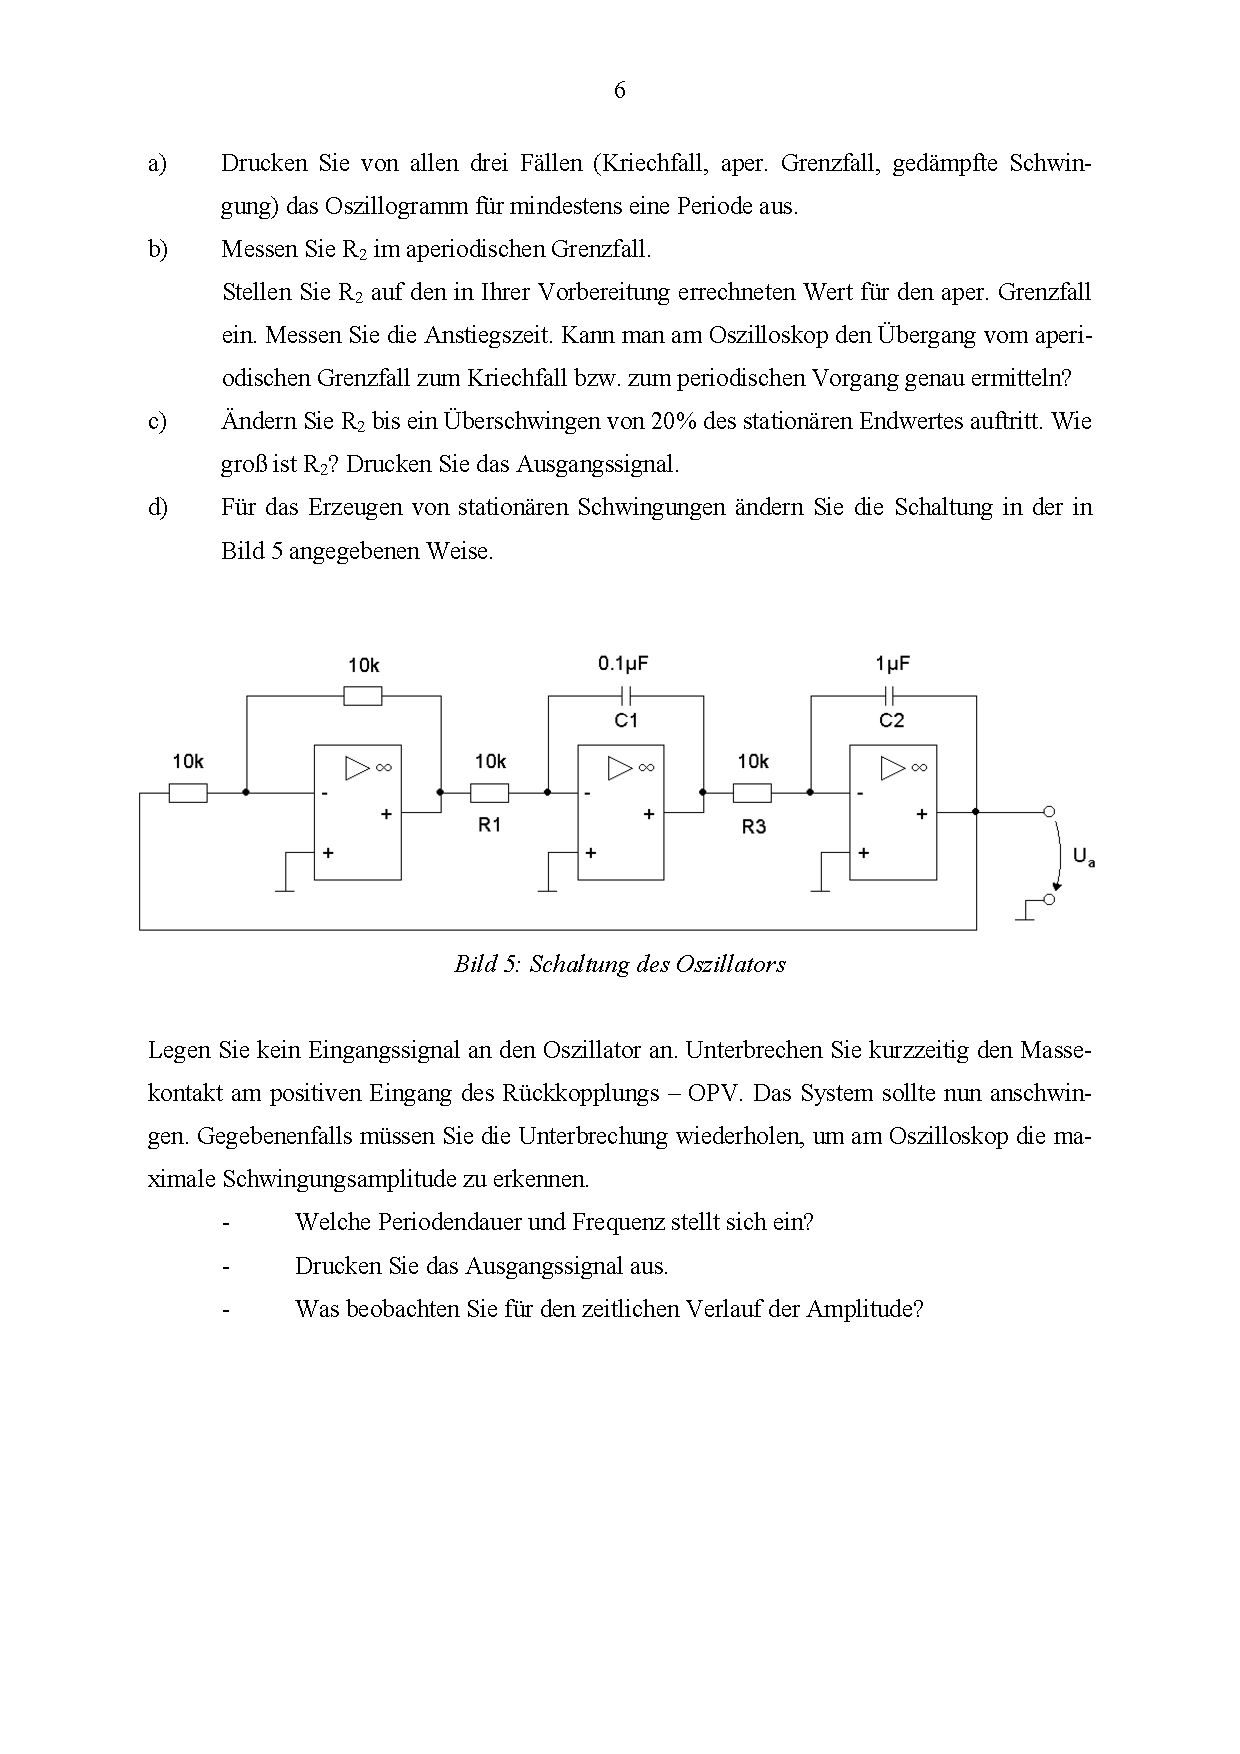
\includegraphics[width=1.0\textwidth]{Bilder/Grundubertragungsglieder im Zeitbereich (verschoben) 6}\newpage
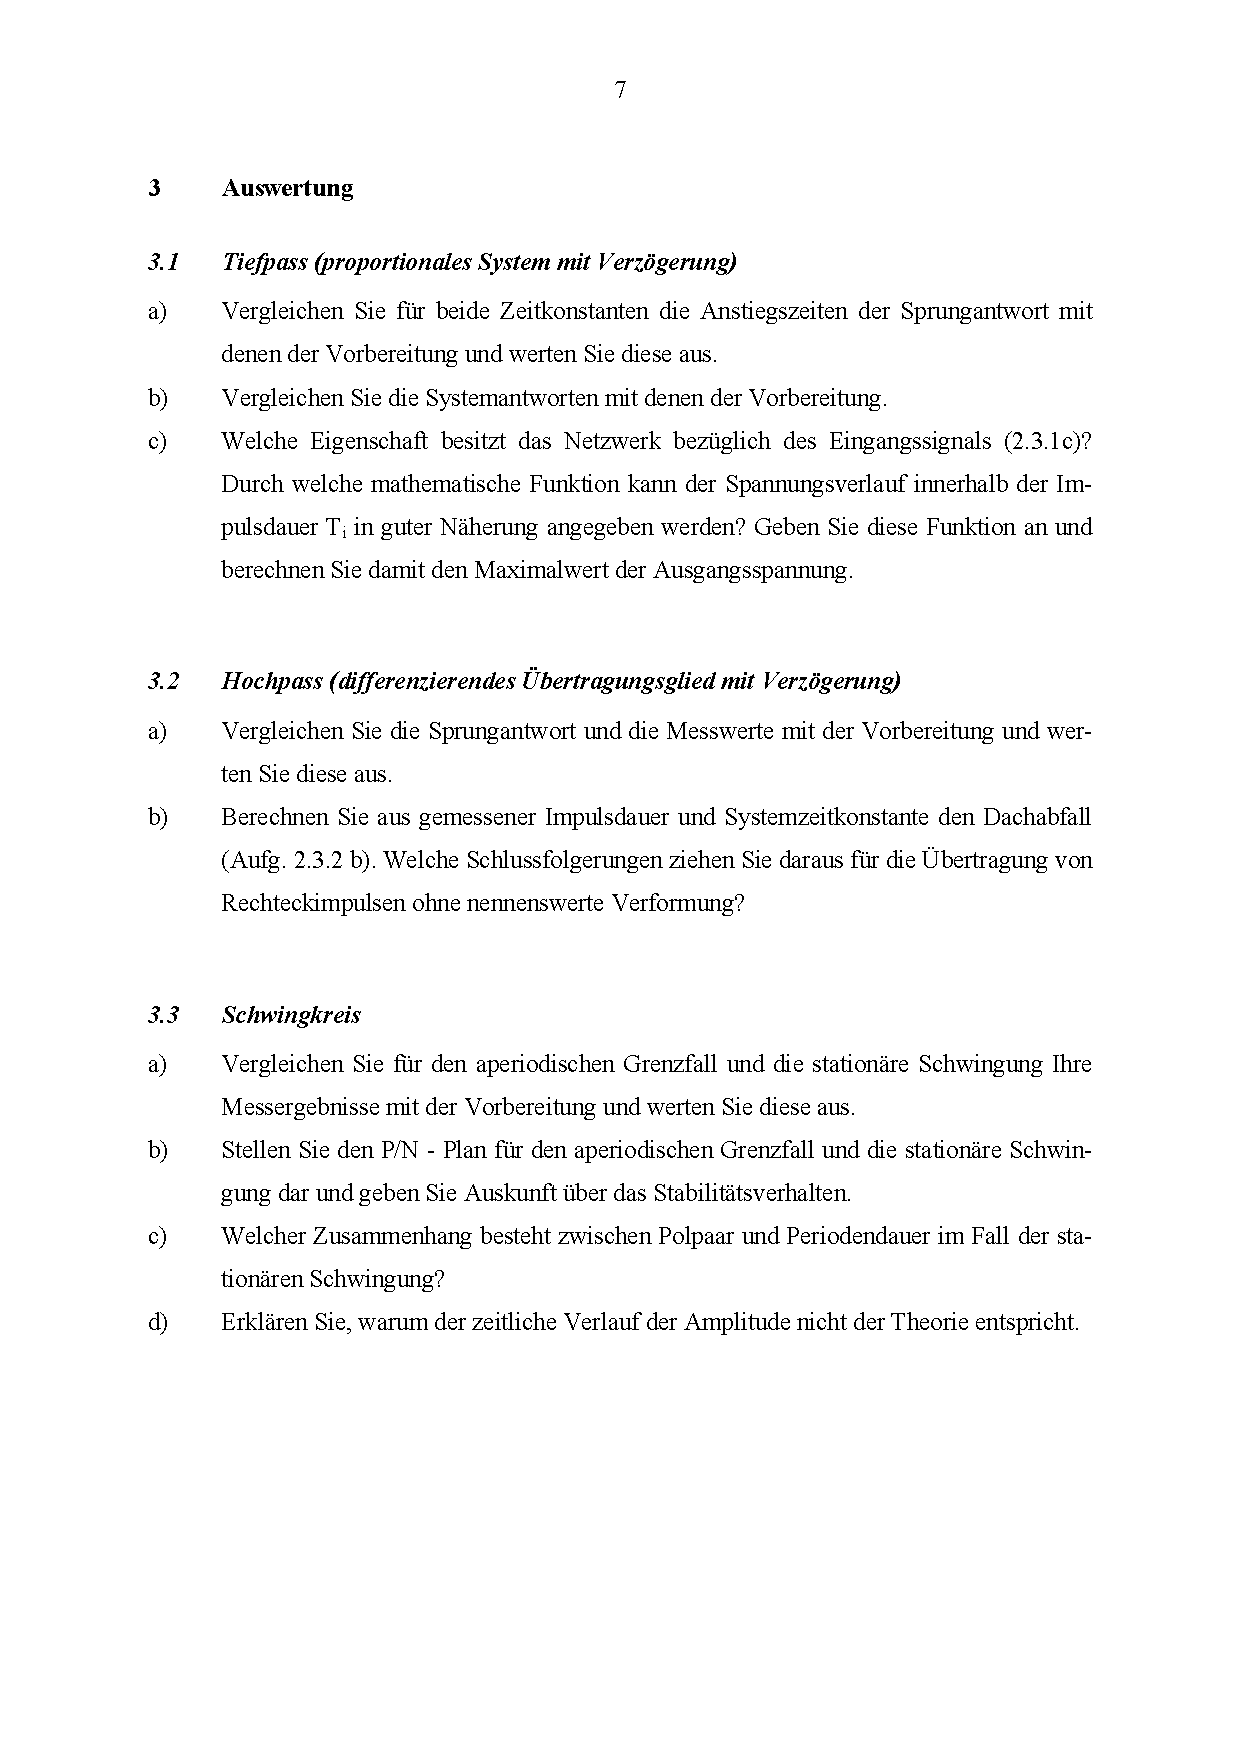
\includegraphics[width=1.0\textwidth]{Bilder/Grundubertragungsglieder im Zeitbereich (verschoben) 7}\newpage


\section{Vorbereitung des Versuches}
\subsection{Ziel und Abgrenzung des Versuches}
\subsection{TheoretischeVoraussetzungen}
\subsection{Vorbereitende Aufgaben}
\subsubsection{Begriffe}
\subsubsection{Tiefpass (proportinales System mit Verzögerung)}
\subsubsection{Hochpass (differenzierendes Übertragungsglied mit Verzögerung)}
\subsubsection{Schwingkreis}
\section{Durchführung des Versuchs}
\subsection{Versuchseinrichtung}
\subsection{Methodische Hinweise}
\subsection{Aufgabenstellung}
\subsubsection{Tiefpass (proportinales System mit Verzögerung)}
\subsubsection{Hochpass (differenzierendes Übertragungsglied mit Verzögerung)}
\subsubsection{Schwingkreis}
\section{Auswertung}
\subsection{Tiefpass (proportinales System mit Verzögerung)}
\subsection{Hochpass (differenzierendes Übertragungsglied mit Verzögerung)}
\subsection{Schwingkreis}


\cleardoublepage

%Einbinden des nächsten Kapitels

\clearpage
\pagenumbering{roman}


\printbibliography[heading=bibintoc,title={Quellenverzeichnis}]

\end{document}
